\documentclass[a4paper,12pt]{book}
\usepackage[utf8]{inputenc}
\usepackage{graphicx}
\usepackage{xfrac}
\usepackage{listings}
\graphicspath{ {./Images/} }

\begin{document}

\author{Spectrecoin Team}
\author{Spectrecoin Team}
\title{White Paper}
\date{11th June 2019\\
	Spectrecoin version 3.0.10}

\frontmatter
\maketitle
\tableofcontents

\setlength{\arrayrulewidth}{.5mm}
\setlength{\tabcolsep}{10pt}
\renewcommand{\arraystretch}{1.5}

\mainmatter
\section{Abstract}
Cryptocurrencies (\textit{digital assets designed to work as mediums of exchange})
permit users to securely send money without trusting any other human intermediary
or any other centralised third-party system or institution, such as a bank, to
verify those transactions\footnote{https://en.wikipedia.org/wiki/Cryptocurrency}.
Instead the strong cryptography and mathematics inherent in the software
algorithms secure the peer-to-peer network and safeguard against forgeries and
ensures transaction finality. The network of participating nodes together
creates the blockchain where all transactions and balances are recorded and
ensures network immutability. This is a truly transforming technology and has
the potential to benefit people across the globe. However, the blockchains in
classic cryptocurrencies (\textit{such as Bitcoin}) are transparent public
ledgers that are accessible to anyone and the full transaction history is
preserved and the blockchain is readily available for analysis\footnote{https://www.respublica.org.uk/disraeli-room-post/2015/03/24/bitcoin-is-not-anonymous/}.
This presents a very serious issue for users online and financial privacy.
Even though the pseudonymous users of classic blockchains are not directly
associated with their real-world identities, every transaction among these
pseudonyms is potentially traceable and every transaction is recorded for
all posterity and for \underline{anyone} to access and view.

In this white-paper, we present \textbf{Spectrecoin}; a cryptocurrency that
uses a range of advanced cryptographic techniques, such as dual-key stealth
addresses and ring-signatures to achieve un-linkable and un-traceable
private and confidential transactions on its blockchain. \textbf{Spectrecoin}
also comprises a novel privacy-preserving consensus mechanism,
‘\textbf{\textit{Proof-of-Anonymous-Stake}}’ that let its users retain
full privacy as they support the network by running the software and
staking their coins. \textbf{Spectrecoin} also protects the user’s online
identity by integrating TOR (\textit{The Onion Router})\footnote{https://www.torproject.org/} 
in the software and is therefore a
comprehensive privacy focused cryptocurrency. \textbf{Spectrecoin} also
retains the ability to conduct ‘\textit{open}’ public transactions
(\textit{much like Bitcoin}) and this may serve certain use cases and
blockchain audit-ability. \textbf{Spectrecoin} provides the best of both
worlds, total privacy and public transactions, without any compromise.
In this paper we present the current technology and functionality of
\textbf{Spectrecoin} to the common reader with some experience and knowledge
of blockchain and cryptocurrencies. We also discuss how we achieve
confidential and privacy maintaining consensus and we discuss what
\textbf{Spectrecoin} aims to achieve in the future. Further references
to explain and expand on certain topics are included within the text as
footnotes.

\chapter{Acknowledgements}
\textbf{Spectrecoin} would not have been possible without the foundations
laid by what came before and in particular the \textit{Bitcoin}
\footnote{https://bitcoin.org/bitcoin.pdf}, \textit{Blackcoin}
\footnote{https://blackcoin.org/blackcoin-pos-protocol-v2-whitepaper.pdf}
and \textit{ShadowCash}\footnote{https://www.cryptoground.com/shadowcash-white-paper}
developers and the work by the authors of the \textit{CryptoNote}
\footnote{https://cryptonote.org/whitepaper.pdf} and \textit{Zerocoin}
\footnote{http://zerocoin.org/} protocol that provided inspiration for
some of the technologies developed for use in Spectrecoin. Although the
Spectrecoin lineage can be traced back through previous projects, open
source software provides inspiration for innovation and progress.
Spectrecoin has taken a particular direction to improve, enhance,
innovate and further develop the unique privacy technology inherent
in its code base. The Spectrecoin developers have also written copious
amounts of original code and developed innovative technology not seen
in any other comparable cryptocurrency.

\section{Disclaimer}
\textbf{The Spectrecoin software} and the source code is being developed 
and maintained by the ‘\textbf{The Spectrecoin Foundation}’
(\textit{a UK registered Community Interest Company, number: 11884217, hereafter
referred to as The Foundation})\footnote{https://beta.companieshouse.gov.uk/company/11884217}.
The Foundation does not hold any personal information on any users of the
Spectrecoin software and will never ask for any identifying information
from any user in order to download and use the software. The Foundation
does not collect any personal data. \textbf{The Foundation will NEVER ask
users for their private keys, wallet / data files or any other information 
that could enable us to access a user’s fund or wallet or identify the
user.} The Foundation does not hold any kind of key / information / data
or have any other means or technology that would enable it to analyse
transactions on the Spectrecoin blockchain with a view to identify any
user. The creation of the Spectrecoin network did not involve any trusted
setup and no personal information was ever collected. Spectrecoin would
immediately disclose any kind of communication or request from any
government or other agency for information of any kind or any action on
our part.
\\
\\
The Foundation understands and appreciates that the Spectrecoin software 
holds and protects your money and we take this responsibility seriously. The
Foundation is doing everything it can to make sure that the network and
the software is as secure as it can be. However, the software comes with
no guarantees and must be considered experimental. In general, confidentiality
and privacy should never be considered as an absolute and users should do their
own due diligence and risk assessment and take whatever measures they deem
appropriate to protect themselves online. When conducting a risk assessment
with regards to your own privacy online; consider that we do not have
conclusive knowledge of any possible adversary’s capabilities or resolve to
achieve their aims. The Foundation does not in any shape or form condone any
illegal activity and Spectrecoin has not been created to facilitate any kind
of illegal activity.
\\
\\
The Foundation is not responsible in any way whatsoever for any lost password,
hacking, acts of God, war, natural disasters or any other unforeseen event
that could compromise the network and cause any loss of funds. The Foundation
cannot be held responsible for any users incompetence or recklessness that may
result in any loss or liability. The current parameters of the software are set
according to how we believe the network should operate, but network parameters
and characteristics could change if deemed necessary. The Foundation will always
work to increase the privacy of the Spectrecoin software, increase the value of
the company and hence the value of your investment. All decisions are made with
this in mind. This is not investment advice and we do not offer any investment
or financial advice.
\\
\\
If you own Spectrecoin and you run a Spectrecoin wallet, it is strongly
recommended that you always keep up to date with developments and always run
the latest version of the software. This is best done by either subscribing
to our Discord server\footnote{https://discord.gg/ckkrb8m} or use 
Blockfolio\footnote{https://blockfolio.com/}.

\chapter{Notes}
Spectrecoin employs well known technology albeit used in creative ways and some parts of the white-paper is to a large degree referencing already published material from various sources. The newly added section on ‘\textbf{\textit{Proof-of-Anonymous-Stake}}’ however is unique to this white-paper and an original Spectrecoin technology. There is no scope in this document to discuss cryptography or mathematics and the author is neither a cryptographer nor a mathematician. The descriptions of cryptographic functions are taken from the relevant source documents that are referenced throughout this document and if you are so inclined you can read up on the details. This is not meant as an academic paper or as a reference document but rather as a brief description of the Spectrecoin network and the underlaying technology used. This document does not intend to contribute to the debate about privacy online and this discussion is beyond the scope of this document. We simply believe that we have an absolute right to privacy in our financial affairs online as we do in the real world and so our ideology is also simple; to provide real decentralised resilient privacy and confidentiality on the blockchain and offer provable private transactions for users. 
\section{Commonly Used Terms}
\begin{description}
	\item[Blockchain:] A shared, immutable ledger for recording the history of transactions in blocks.
	\item[Block:] A defined data structure that contains a record of transaction data and other values.
	\item[XSPEC:] The symbol (ticker) for Spectrecoin and also the name of the public coins on the blockchain.
	\item[SPECTRE:] The name used for the private coins on the Spectrecoin blockchain.
	\item[UTXO:] Unspent Transaction Output that can be spent as an input in a new transaction.
	\item[ATXO:] UTXO that can be spent as in input in a private transaction using a ring signature.
	\item[Keyimage:] A unique value associated with a specific ATXO calculated using a private key.
	\item[Spent (UTXO):] A UTXO is spent when it has been ‘consumed’ as an input in a new transaction.
	\item[Spent (ATXO):] An ATXO is spent when the related ‘keyimage’ has been included in a valid ring signature.
	\item[Hash function:] A mathematical one-way function that generates fixed size data from an arbitrary input.
	\item[Hash value:] A numeric \textbf{value} of a fixed length that uniquely identifies the data input in a hash function.
	\item[Block hash:] The hash of a block's header.
	\item[Kernel Hash:] A hash value used in Proof-of-Stake.
	\item[Mixin:] A chaff or dummy ATXO not being spent in a current transaction, used in a ring signature.
	\item[TOR:] The Onion Router. A layered network that attempts to hide your IP address.
	\item[VIN:] The ‘collection’ of input data for a transaction, including the UTXOs/ATXOs to be consumed.
	\item[VOUT:] The ‘collection’ of output data for a transaction, including the new UTXOs/ATXOs generated.
	\item[PoS:] Proof-of-Stake. A consensus mechanism introduced with Peercoin
	\item[PoSv3:] Proof-of-Stake v3. Consensus mechanism developed by the Blackcoin developers.
	\item[PoAS:] Proof-of-Anonymous-Stake. Privacy consensus mechanism introduced by the Spectrecoin developers.
\end{description}

We will use some screenshots from the Spectrecoin block
explorer\footnote{https://chainz.cryptoid.info/xspec/} to show examples of
transactions and to explain some of the features. The block explorer
is not custom made for Spectrecoin and will always show ‘\textit{XSPEC}’
as the designation behind a value. When this is preceded by the word
‘\textit{Anonymous}’ it designates a SPECTRE value.

\begin{figure}[ht]
	\caption{Example of a parametric plot ($\sin (x), \cos(x), x$)}
	\centering
	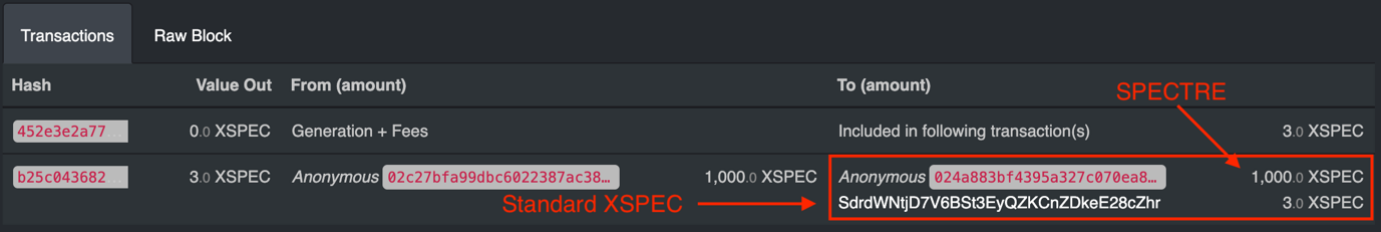
\includegraphics[width=\textwidth]{ExampleStakingTransaction.png}
\end{figure}


References are designated by superscript (numbers) and relate to the relevant
footnotes and links at the bottom of each page. Please follow the links to
explore certain topics in more detail.

\chapter{Introduction}
Spectrecoin strives to provide real-world confidential and private transactions that will withstand any kind of blockchain analysis by the most hostile and determined attacker. We will achieve this through constantly working to test and audit the source code and seek to improve the privacy of our transactions and develop new technology. With the recent introduction of a totally private staking protocol, ‘Proof-of-Anonymous-Stake’, you can now also keep your money private and earn a healthy interest by running the Spectrecoin software. In this context it is important to understand and appreciate that any cryptocurrency aiming for private transactions will be up against increasingly sophisticated ways to analyse the blockchain and increasingly sophisticated analytical tools. It is in fact an arms race and we must therefore not sit back and claim that our privacy is forever unbreakable, but we must conduct an honest and fearless audit of the algorithms and methods behind the private transactions and discover our own weaknesses and vulnerabilities. We then need to work to improve our code to stay at the front of the arms race. We will then become a trusted and functional cryptocurrency with real-world privacy, one of the few out there, beyond just the hype. It is therefore also important that our users understand what is real and what is not when it comes to online privacy.
\section{Spectrecoin Basic Properties}
The Spectrecoin software is encompassing and integrating the following:

\begin{description}
	\item[Bitcoin Core] (core technology of the Spectrecoin block-chain)
	\item[Proof-of-Stake.v3 (PoSv3)] (secure ‘open’ consensus mechanism 
	for XSPEC public coins)
	\item[Proof-of-Anonymous-Stake (PoAS)] (secure private consensus 
	mechanism for SPECTRE private coins)
	\item[Private transactions] (using dual-key stealth technology and 
	ring signatures for SPECTRE)
	\item[TOR] to hide your real IP address (all Spectrecoin nodes run as 
	hidden services)
	\item[OBFS4] to hide the fact that you are using TOR to avoid censorship
\end{description}



\subsection{Core Specification}

\begin{tabulary}{\textwidth}{L|J}
	\hline
	Genesis block 				& Block \#1 mined on 20/11/2016 (later transition to PoS only)\\
	\hline
	Distribution  				& ICO that raised 16 BTC w/ subsequent distribution in early 2017\\
	\hline
	Ticker 						& XSPEC\\
	\hline
	Initial supply 				& 20,000,000 XSPEC\\
	\hline
	Network outputs (public) 	& XSPEC – public coins\\
	\hline
	Network outputs (private)	& SPECTRE – private coins\\
	\hline
	Consensus (XSPEC) 			& Proof-of-Stake v.3 (PoSv3)\\
	\hline
	Consensus (SPECTRE) 		& Proof-of-Anonymous-Stake (PoAS)\\
	\hline
	Difficulty retarget 		& Every block\\
	\hline
	Target block time 			& 96 seconds\\
	\hline
	Block reward (PoSv3) 		& 2 XSPEC\\
	\hline
	Block reward (PoAS) 		& 3 SPECTRE\\
	\hline
	Coin maturity (confirmations) 	& 450 for stake reward / 10 for SPECTRE / 6 for XSPEC\\
	\hline
	Max supply 					& No max supply (see illustrations on page 8)\\
	\hline
	Inflation 					& Decreasing over time tending to zero\\
	\hline
	Code repository 			& https://github.com/spectrecoin/spectre\\
	\hline
	Supported platforms / OS 	& MS Windows, OSX, Linux, Raspberry Pi\\
	\hline
	Website 					& https://spectreproject.io/\\
	\hline
	Block explorer 				& https://chainz.cryptoid.info/xspec/\\
	\hline
\end{tabulary}

%\pagebreak[4]
\vspace{15mm}

It is important to understand that the total ‘\textit{outstanding}’ amount is the sum
of \linebreak XSPEC + SPECTRE. On the next page we have projected both a minimum and a
maximum inflation rate and total ‘\textit{outstanding}’ amount of XSPEC + SPECTRE over
20 years. The real value of the total ‘\textit{outstanding}’ amount will depend on the
ratio of XSPEC / SPECTRE created by the two different consensus mechanisms
over time. The minimum values represent a scenario where 100\% of the blocks
are created by PoSv3 and the maximum values represent a scenario where 100\%
of the blocks are created by PoAS.

\begin{figure}
	\centering
	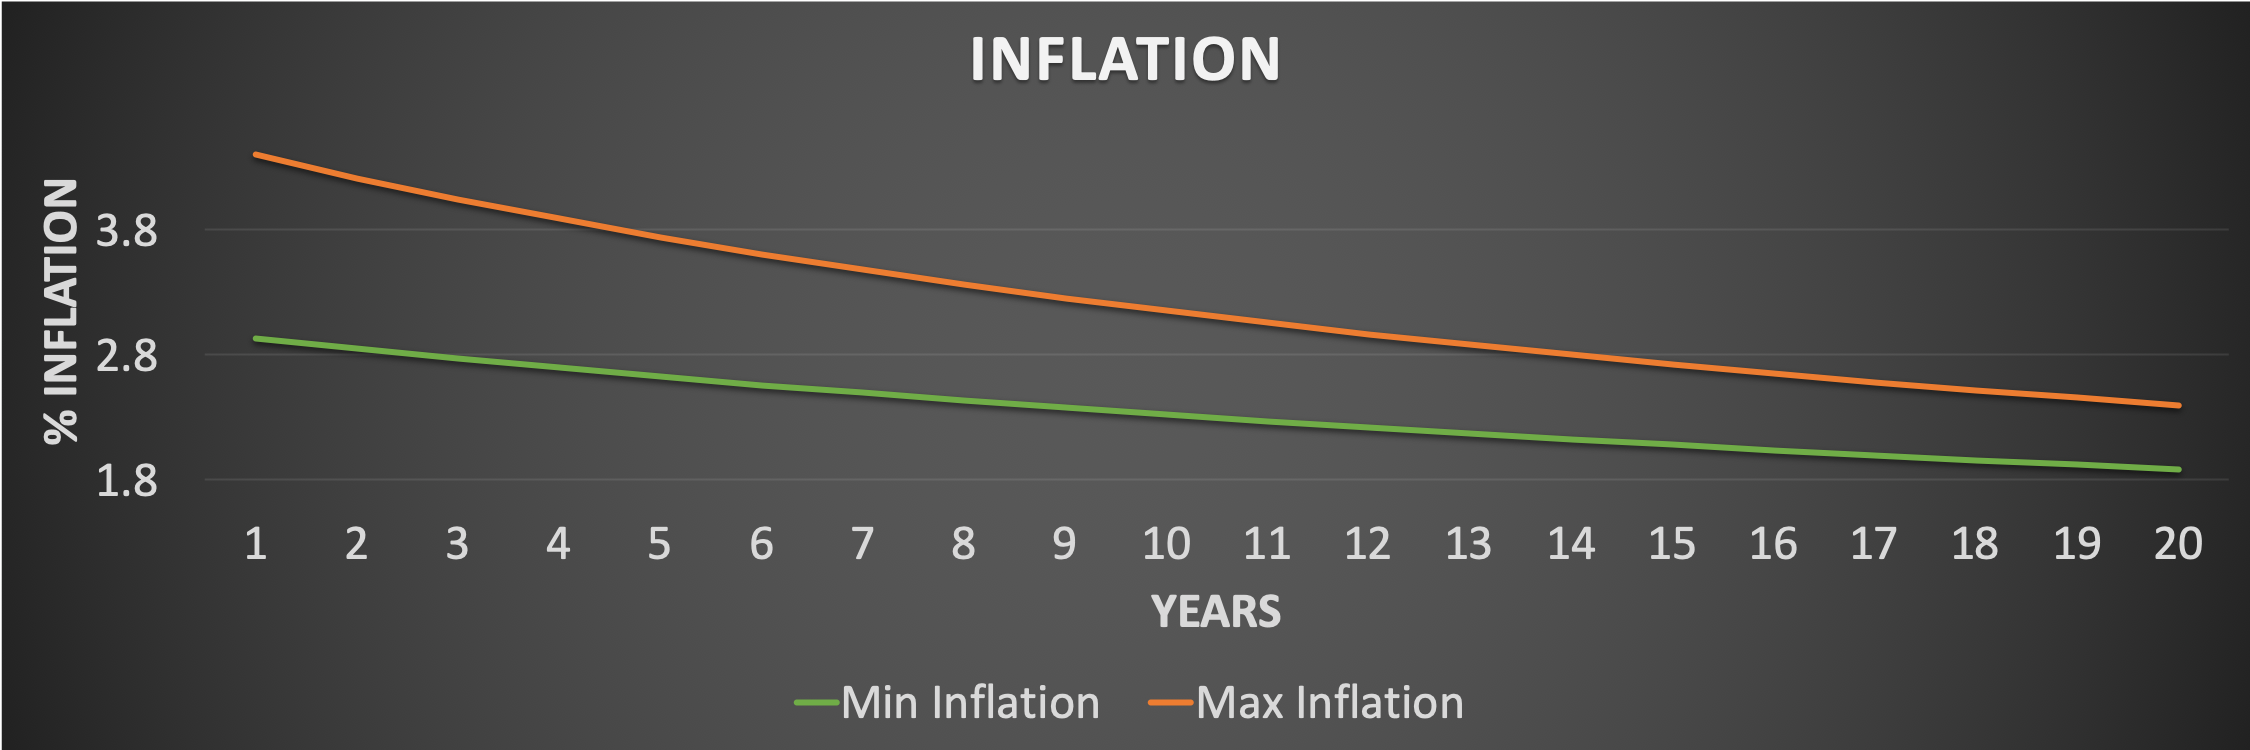
\includegraphics[width=\textwidth]{inflation.png}
	\caption{Min inflation rate after 20 years = 1.88 - Max inflation 
	rate after 20 years = 2.40 }
\end{figure}



\subsection{Inflation rate over 20 years}



There are different strategies employed by different cryptocurrencies around 
Inflation\footnote{\textit{Spectrecoin differs from Bitcoin and some other 
cryptocurrencies in that we have a constant coin generation scheme 
but a relative inflation that tends to zero over time. There will 
always be an incentive to stake Spectrecoin and the system will never 
rely on fees alone to provide this incentive. It is beyond the scope 
of this paper to have an in-depth discussion about inflation and money 
supply and the nature of money and currencies. Spectrecoin can be seen 
as a ‘medium of exchange’ and the aim is that Spectrecoin will be used 
to buy/sell goods and other fiat currency in its intended use in future 
online cash transfers. Economists discuss and debate this point but some 
level of inflation and value creation appears to be beneficial for long 
term adoption and will prevent Spectrecoin from the potential dangers of 
entering a ‘deflationary spiral’ relaying on fees alone to sustain the 
Spectrecoin ecosystem.}}. There doesn’t seem to be a consensus amongst 
scholars of what might be ‘\textit{the best}’ strategy.



\subsection{Total supply (‘outstanding’ amount) over 20 years}


\begin{figure}[ht]
	\centering
	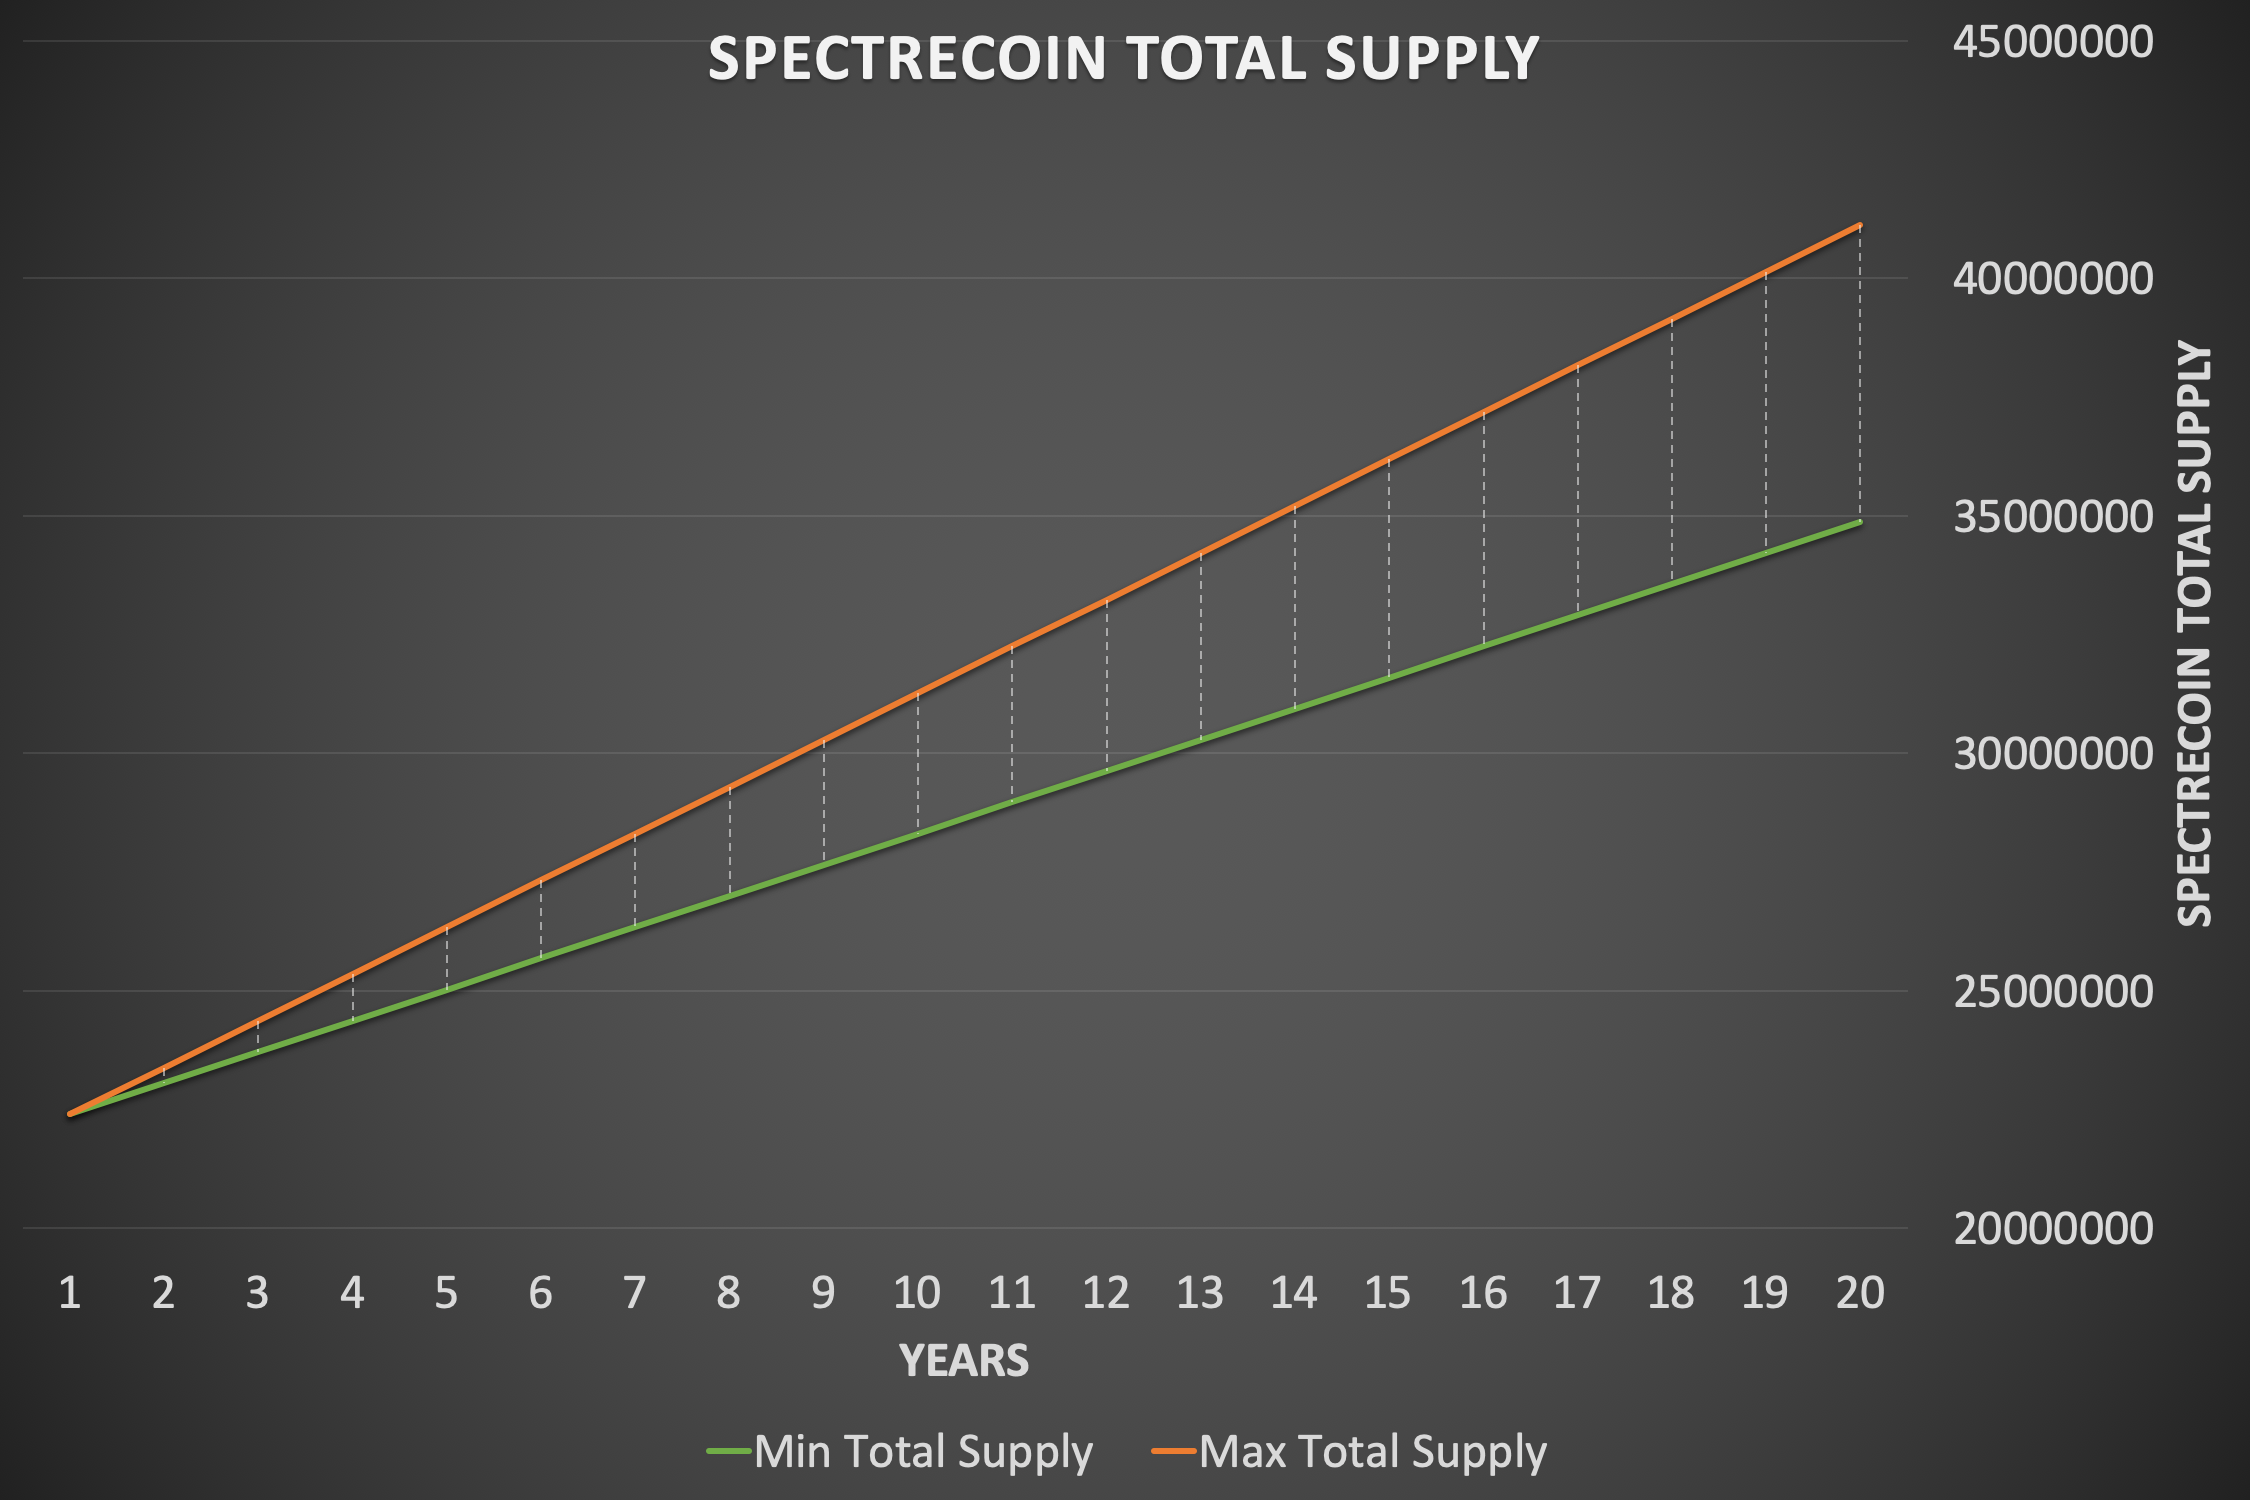
\includegraphics[width=\textwidth]{supply.png}
	\caption{Min supply after 20 years = 34,883,000 XSPEC+SPECTRE - Max 
		supply after 20 years = 41,124,500 XSPEC+SPECTRE}
\end{figure}



The block explorer\footnote{https://chainz.cryptoid.info/xspec/} allows you 
to explore the Spectrecoin blockchain.



\subsection{Maturity}
The maturity calculations have changed such that the minimum maturity for
staking and for spending stakes has been increased from 288 to 450 blocks.
This is approximately 96 seconds * 450 = 12 hours and hence the 8-hour
maturity rule for staking has been removed. Also, note that the updated
maturity rule is also considered for all ATXOs used in the ring signature
of the staked VIN.



\subsection{Reward and Fee Handling}
The stake reward for a PoAS block is 3 SPECTRE and 2 XSPEC for a PoSv3 block.
The fees are the same for both XSPEC and SPECTRE transactions.



\subsection{Proof-of-Stake vs. Proof-of-Work}
Spectrecoin uses both PoSv3 and PoAS algorithms to keep the network consensus
and to secure and confirm transactions. Both PoSv3 and PoAS appear to be more
resilient against various attacks that could be instigated against a
Proof-of-Work (PoW) system like Bitcoin, Litecoin and DASH for example.
It is also known that PoW systems are susceptible to so called 51\% attacks
where a sufficiently funded and motivated attacker can “\textit{take control}” over
the network and generate double spend transactions\footnote{https://www.crypto51.app/}. 
It is more difficult to attack a PoS system in this way as it would be infeasible 
to acquire the majority of Spectrecoin in circulation and doing so would undermine 
the value and remove the incentive for the attack in the first place. There are 
obviously other attack vectors, such as the recently discovered so called 
“\textit{Fake Stake}” attack against 
PoSv3\footnote{https://medium.com/@dsl\_uiuc/fake-stake-attacks-on-chain-based-proof-of-stake-cryptocurrenciesb8b05723f806}. 
This has since been fixed by the Spectrecoin developers and Spectrecoin is no 
longer susceptible to such an attack.



It is also well known that large PoW driven networks expend huge amounts of
energy and appears to lead to some level of centralisation of mining power
due to the huge expense involved in mining new blocks. In a recent research
paper entitled “\textit{The Bitcoin Mining Network - Trends, Composition, Average
Creation Cost, Electricity Consumption \& Sources}” by Christopher Bendiksen
\& Samuel Gibbons of CoinShares 
Research\footnote{https://coinshares.co.uk/\#mailmunch-pop-792759}, 
it was found that the Bitcoin network expends more energy than the whole 
country of New Zealand.



The report calculated that the global Bitcoin mining industry draws 4.7GW of
power every second. Hashing computations for the Proof-of-Work algorithm
consumed 4.3GW, up 0.4GW from the last CoinShares report in November 2018.
Based on these figures, researchers calculated \textbf{an annual consumption of
41TWh of electricity}. That’s roughly 2.2TWh more than New Zealand – a country
of 4.7M people – consumed in 2017, according to the country’s Electricity
Authority\footnote{https://www.ea.govt.nz/}.



In comparison, Spectrecoin will run on a standard Raspberry Pi and in addition
to all the privacy features, Spectrecoin is also truly eco-friendly, sustainable
and ‘\textit{green technology}’. The estimated loose upper bound, \textbf{annual 
consumption for a Raspberry Pi running Spectrecoin is 16.6kWh}.

\vspace{5mm} %5mm vertical space

Bitcoin network:\\
$41 TWh = 41*1012 Wh = 41,000,000,000,000 Wh$

\vspace{5mm} %5mm vertical space

Spectrecoin node:\\
$16.6 KWh = 16.6 * 103 Wh = 16,600 Wh * 1000 (nodes) = 16,600,000 Wh$

\vspace{5mm} %5mm vertical space

That means that the whole \textit{Bitcoin network consumes almost 2.5 million times
more energy than what an imaginary Spectrecoin network would consume}, assuming
1000 Spectrecoin Raspberry Pi nodes.




In summary, the PoSv3 / PoAS protocols are both potentially more secure,
immensely more energy efficient and provides for better decentralisation.
It is beyond the scope of this paper to discuss this further and there are
various discussions around the internet if you are interested in the PoW vs.
PoS debate.



In the next sections we will explore the different aspects of Spectrecoin in
more detail. We start on the next page with a detailed introduction to the
Spectrecoin privacy features before we go on to discuss Proof-of-Stake v3
(PoSv3) in detail. We move on to explain the privacy features and the new
Proof-of-Anonymous-Stake (PoAS) protocol.
\chapter{Spectrecoin Privacy Features}
Before we go on to explain some of the features and technologies of
Spectrecoin in more detail, we will give you a short overview of the
privacy technology used. The Spectrecoin blockchain is a ‘dual-coin’
system or a system where two distinct types of transaction outputs can
exist in the same block. Both non-private or standard UTXOs (hereafter
referred to as public coins or XSPEC) and private coins or ATXOs (hereafter
referred to as private coins or SPECTRE) exists side by side in the
block-chain. Transactions can be carried out with both public and private
coins and they are interchangeable and independent. We introduce the terms
XSPEC for the public coins spent in standard UTXO based transactions and
SPECTRE for the private coins spent in a confidential ATXO based
transactions using ring signatures. XSPEC is used in the PoSv3 consensus
mechanism and SPECTRE is used in the PoAS consensus mechanism.



\section{Dual Coin System}
The private coin ‘subsystem’ was inspired by the principles of the Zerocoin
protocol which can be summarised as ‘Anonymity by destruction / creation of
basecoins’, i.e. destroy / consume one base unit, create a private token
and create a proof that the user owns it and the system later agrees to
re-create one base coin from that proof when requested. The Zerocoin protocol
utilises a so called zero-knowledge proof (ZKP) to create the private coins
and to prove ownership. Zerocoin is computationally intense and requires a
trusted setup and we have recently seen that the Zerocoin protocol can be
subject to certain attacks due to what can be described as flaws in the
theory and implementation16. Some well-known Zerocoin based cryptocurrencies
such as Zcoin, PIVX and NIX were forced to shut down their privacy system and
work to implement fixes.



The Spectrecoin network instead employs dual-key stealth address cryptography
to facilitate the creation of privacy maintaining SPECTRE coins on the
blockchain whilst consuming XSPEC. This is done without the trusted setup
required for Zerocoin and without using the computationally intense Zerocoin
cryptographic methods. Where the Zerocoin protocol use ZKP to anonymise and
unlink the transactions, the Spectrecoin network use ring signatures17 \& 18.



\begin{figure}[h]
	\caption{Example of a parametric plot ($\sin (x), \cos(x), x$)}
	\centering
	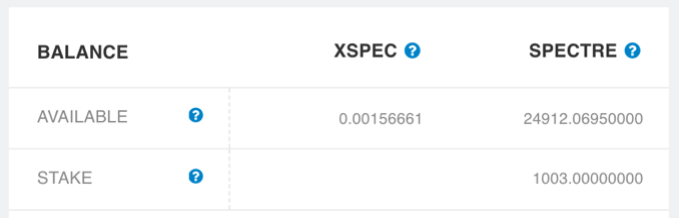
\includegraphics[width=0.5\textwidth]{Wallet-BalanceDualCoin.png}
\end{figure}



The ‘dual-coin’ system can be seen as a feature allowing for complete
transparent transactions and network audit functions if needed but
without any privacy indebted overhead such as resource intensive
calculations. Privacy maintaining SPECTRE can ONLY be created by
consuming XSPEC at this time and the total supply on the network
will always be transparent. There is no ‘bleed through’ between the
two types of transaction outputs and no compromise in privacy.



\section{XSPEC/SPECTRE Conversion}
Each user can convert (non-private) XSPEC coins into (private) coins, SPECTRE.
Users can then send SPECTRE to other users and split or merge the SPECTRE they
own in any way that preserves the total value. Once SPECTRE has been created
and matured the user will also be able to stake in private through the PoAS
protocol. Users can also convert SPECTRE back into XSPEC, though in principle
this is not necessary: all transactions can be made in terms of SPECTRE.



Your wallet will show your XSPEC balance, your SPECTRE balance and on top the
total balance.



The core privacy technology used in Spectrecoin is: Recipient privacy: Stealth
addresses are used to protect the recipient’s privacy. (SPECTRE only) Sender
privacy: Ring Signatures are used to protect the sender’s privacy. (SPECTRE
only) IP address privacy: All Spectrecoin nodes run as TOR hidden services to
protect users IP address. Un-traceability: for each incoming transaction all
possible senders are equiprobable. (SPECTRE only) Un-linkability: for two
outgoing transactions it is impossible to prove the same receiver. (SPECTRE
only)



Now let’s have a look at the different features in some more detail in the
following sections. We aim to briefly explain the background and nature of
stealth addresses and ring-signatures and how this is used in Spectrecoin.

\section{Stealth Addresses}
Before we go on to explain what stealth technology is and how it is used in
Spectrecoin we need to get some background and some knowledge about how
standard UTXO transactions might be de-anonymised and why stealth technology
came to be used to counter this issue. It will also become apparent why
stealth address technology in itself is not sufficient to provide reasonable
privacy.
\\
\\
\noindent
The Spectrecoin blockchain is based on the design from Bitcoin Core 
(\textit{except the consensus mechanisms}) and in both systems there are 
$1.46 \ast 10^{48}$ possible receiving addresses. This is an extremely 
large number and it would give every person on Earth $2.05 \ast 10^{38}$ 
different receiving addresses to use. The fact that it is possible
to re-use an address more than once can be considerd a fluke and is not by
design.
\\
\\
\noindent
First, let’s have a quick look at how a UTXO blockchain might be deanonymized.
The three major factors that can reduce privacy for the user and are exploitable
through transaction graph analysis are \textit{address re-use, change addresses 
and the merging of outputs}.
\\
\\
\noindent
Address re-use is treating XSPEC addresses like a bank account where a single
address is used for multiple transactions. XSPEC addresses are not designed to
be used in this way. There are in fact no restrictions on the number of XSPEC
addresses one person can use and for each transaction a new XSPEC address should
be created.
\\
\\
\noindent
When addresses are re-used, all other transactions performed by that address
can be seen by examining the blockchain. If you are aware of a transaction
made by a person of interest and that transaction comes from the same address
by which this person receives all their payments, then their balances can
easily be determined. You will also be able to look back at the history of
that address, following the chains of transactions, to ascertain what other
information can be extracted.
\\
\\
\noindent
Address re-use also weakens the security of the coins stored in those addresses.
Transaction signing requires 256 bytes of random data (r-value) so that the
private key cannot be reverse engineered. If the \textit{r-value} is not truly random
then the private key can be determined, which can be used to sign other
transactions for that particular address. This attack can be negated by
not re-using addresses, as once a transaction is signed from an address,
it remains empty.
\\
\\
\noindent
Furthermore, each input in a standard transaction must be a full UTXO
from a previous transaction as UTXO’s cannot be partially spent. This
means that if you spend / send less than a full UTXO you will generate
an output that is your change address. Therefore, an attacker examining
the blockchain may generally assume that one output in any transaction
belongs to the creator of the transaction.
\\
\\
\noindent
Also, if a transaction is generated where two or more UTXOs are pooled
together to create the total input required an assumption can be made
that the addresses merged together belongs to the same person.
\newpage
\noindent
Let’s then introduce \textbf{\textit{Stealth Address techniques}} which 
allow public keys appearing in the blockchain to be fully disconnected 
from “\textit{stealth}” public keys which can be publicised by a 
payee\footnote{https://www.scitepress.org/Papers/2017/62700/62700.pdf}. 
The public “\textit{stealth}” keys publicised serve as a 
“\textit{master public key}” from which “\textit{ephemeral public
keys}” are derived. The “\textit{stealth}” public key is never recorded in the
blockchain. This enables the payee to receive infinite un-linkable
payments by publicising only one stealth address. The problem of address
re-use is therefore 
solved\footnote{http://www.nicolascourtois.com/bitcoin/paycoin\_privacy\_monero\_6\_ICISSP17.pdf}. 
\textbf{A Stealth address therefore is a privacy technique that protects 
the privacy of the recipient.} The first stealth address technique was 
invented by a user known as ‘\textit{bytecoin}’ in 2011 in the Bitcointalk 
forum. Later improvements to stealth tech were proposed by van Saberhagen 
in 2013/14 and by Peter Todd in 2014.
\\
\\
\noindent
The original stealth technology had various problems and on 02/08/2014 one
of the ShadowCash developers known as ‘\textit{rynomster}’ announced a 
first fully working implementation of stealth address technology known as 
“\textit{dual-key stealth addresses}” that solved some of the issues in 
previous proposals. A “\textit{dual-key stealth address}” has two public 
keys and solves certain problems associated with previous schemes. For a 
full and in-depth explanation of stealth addresses see the paper cited below.
\\
\\
\noindent
(\textit{Courtois N. and Mercer R. (2017). Stealth Address and Key Management
Techniques in Blockchain Systems. In Proceedings of the 3rd International
Conference on Information Systems Security and Privacy ISBN 978-989-
758-209-7, pages 559-566. DOI: 10.5220/0006270005590566})
\\
\\
\noindent
The use of dual-key stealth addresses provide privacy for the receiver of
funds and introduces various forms of un-linkability:

\begin{itemize}
	\item It is hard to	link different public keys/addresses of the same user,
	\item It is hard to	link different transactions of the same user,
	\item It is hard to link the sender to the recipient.
\end{itemize}

\subsection{Limitations of Stealth Addresses}
As mentioned above, stealth addresses generate a new standard address for
every payment but if you receive for example 10 transactions using your
stealth address you will have 10 UTXOs available to form further
transactions. If you then use some or all of the UTXOs to form a transaction
an observer will be able to link the UTXOs together and assume that they all
belong to one user (\textit{merging of outputs}). Furthermore, an attacker could
create a number of dust transactions with a stealth address and then monitor
the blockchain to see if the user ever joins those UTXOs together or with
others, in order to make an input to a higher value transaction in the future.
Blockchain analysis can easily link this. \textbf{This is the reason why any
cryptocurrency that relies on stealth addresses ONLY is not private.}
\newpage

\subsection{Anonymous Spectrecoin Conversion}
Dual-key Stealth technology is used in the process to create anonymous 
\textbf{SPECTRE} by consuming the equivalent value of \textbf{XSPEC}. The 
creation of \textbf{SPECTRE} involves the creation of an ATXO with a 
bundled one-time key-pair that will allow that ATXO to be ‘\textit{spent}’ 
by providing a valid ring signature using your remaining public key 
corresponding to the ATXO you previously created and the corresponding 
‘\textit{keyimage}’\footnote{https://monero.stackexchange.com/questions/2883/what-is-a-key-image}. 
The fact that an ATXO has been ‘\textit{spent}’ is only known to the sender 
and an observer cannot determine if the ATXO has been ‘\textit{spent}’.



\subsection{Keyimage}
The ‘\textit{keyImage}’ is the result of a cryptographic one-way function derived
from a user’s one-time keypair. The ‘\textit{keyimage}’ is unique to the ATXO
contributing the value to the new ATXO being created in an anonymous
transaction. The ‘\textit{keyimage}’ is then recorded in the blockchain to prevent
double spends, but without revealing which ATXO is the value-contributing
member in the ring signature. Although the ‘\textit{keyimage}’ is recorded in the
blockchain it cannot be reverse engineered due to the one-wayness of the
cryptographic function that generated it. The calculation of the ‘\textit{keyimage}’
includes the users private key associated with the ATXO being ‘\textit{spent}’.
Hence, if the user tries to spend the same ATXO again the same ‘\textit{keyimage}’
will be generated and the system will reject the transaction as that
‘\textit{keyimage}’ has been seen before.
\\
\\
The following SPECTRE denominations are possible:
\\
$1000, 500, 400, 300, 100, 50, 30, 10, 5, 4, 3, 1, \\0.5, 0.4, 0.3, 0.1, 0.0(000000)5, 0.0(000000)4, 0.0(000000)3, 0.0(000000)1$
\\
\\
\noindent
We have seen how the use of stealth address tech can be used to solve the
problem of address re-use and to create un-linkable transactions. Now, we
still have the problem of UTXOs being linked together in future transactions.
To resolve this issue Spectrecoin employs the use of ring signatures in
transactions formed by ATXO outputs using \textbf{SPECTRE}.

\section{Ring Signatures}
In a standard UTXO transaction the sender signs the transactions using his/her
private key and the signatory can be explicitly determined and identified. In
cryptography, \textbf{a ring signature} is a type of digital signature that can be
performed by any member of a defined group of users that each have the required
keys. A distinctive \textbf{ring signature} is produced through a process that combines
the keys of all possible signers and other values and which are then subject to
a hash function.
\\
\\
\noindent
In cryptography a ring signature is a form of a \textit{non-interactive 
zero knowledge proof}\footnote{https://en.wikipedia.org/wiki/Non-interactive\_zero-knowledge\_proof}. 
In layman’s terms, what this means is simply that you can prove the
correctness of a statement/transaction to a verifier without leaking any additional
information by just using a shared common reference string (\textit{public key}).
This system must include cryptographic completeness, soundness and zero-knowledge.
\\
\\
\noindent
\underline{Completeness} means that if the statement is correct, then the verifier will
always accept. \underline{Soundness} is a property of such a system that requires that
no prover can make the verifier accept a false or incorrect statement. If the
statement is incorrect or false, then the verifier will always reject. The
last part is \underline{zero knowledge}. It is not possible to gain any extra information
from the proof itself for any malicious verifier except for the correctness of
the statement.
\\
\\
\noindent
This offers a group member a level of anonymity not attainable through generic
digital signature schemes. This is a property known as ‘\textit{plausible deniability}’,
or anonymity with respect to an anonymity set. With a ring size of 10 for example
there are 10 possible signatories, i.e. 10 public keys and an observer cannot
determine which one corresponds to the \textbf{SPECTRE} spent in the transaction. This
is only known to the sender. This protects the privacy of the sender. With every
transaction using a ring-signature the network ‘\textit{transactional entropy}’ increases
and it becomes increasingly hard to link input/output on the blockchain.
\\
\\
\noindent
Look at it like this; scattered along the Spectrecoin blockchain are ATXOs of
various denominations from 1000 to 0.00000001 SPECTRE. These ATXOs may be spent
or unspent but this cannot be determined by an observer. The proof of an ATXO
being spent is formed on an ad-hoc basis through the creation of a ‘\textit{keyimage}’
and there is nothing contained within the data of the ATXO itself or the
transaction data written to the blockchain that signifies if it has ever been
‘\textit{spent}’. In a standard UTXO transaction on the other hand an observer can
explicitly determine that an UTXO has indeed been spent to create a new UTXO.
\\
\\
\noindent
See the illustrations on the next page to visualise the difference between an
UTXO and ATXO.
\newpage



\subsection{Standard UTXO transaction}

\begin{figure}[ht]
	\centering
	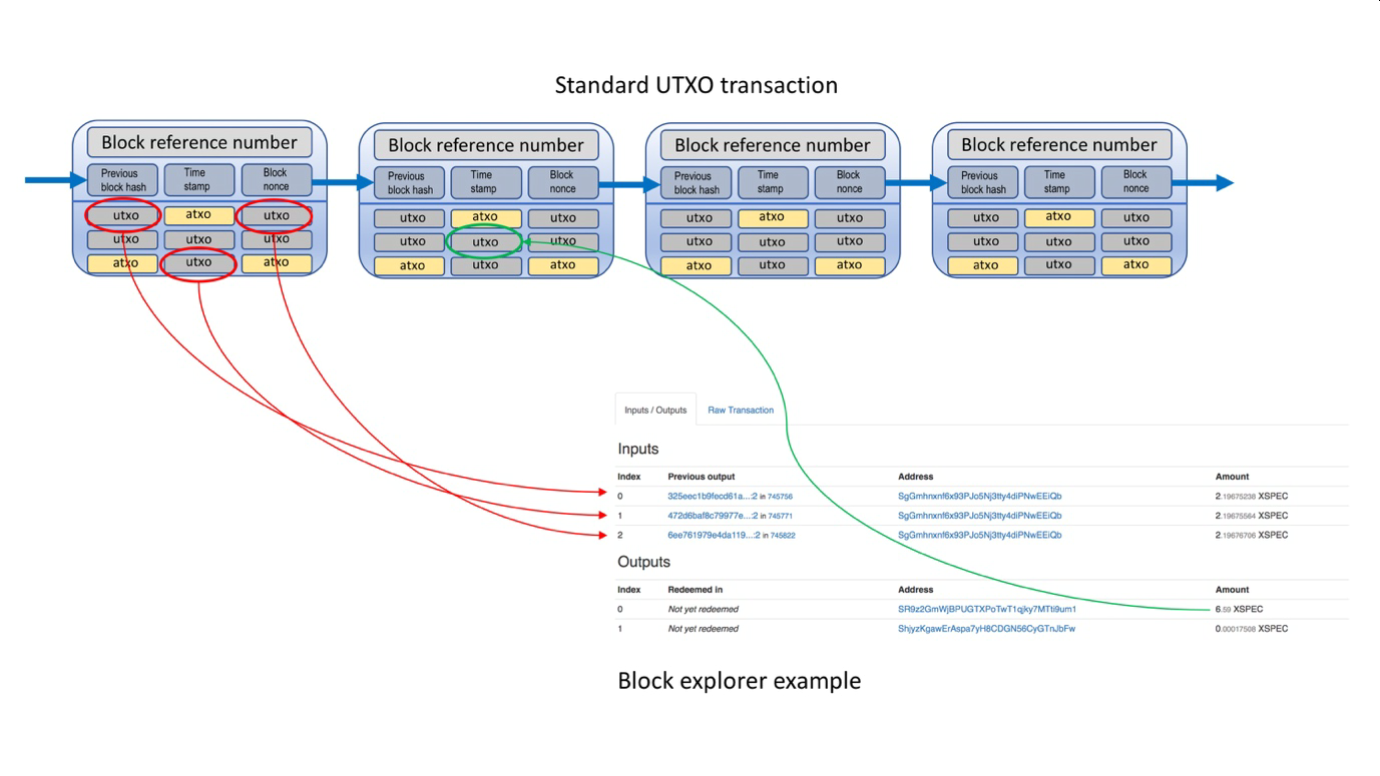
\includegraphics[width=\textwidth]{Std-UTXO-Transaction.png}
	\caption{Standard UTXO transaction}
\end{figure}

\noindent
On the blockchain there is a \textbf{\underline{direct}} correlation
between the inputs and the outputs, and all the transactions can be 
traced back to the genesis transactions. This is still the case even 
if a mixing strategy is used, such as in DASH. There are increasingly 
sophisticated methods to analyse blockchain data and this is a growth 
industry. You should consider any standard UTXO transactions to be 
non-anonymous and public, whether with Spectrecoin or Bitcoin.



\subsection{Anonymous ATXO transaction}

In the Spectrecoin software we talk about ring sizes and this refers to the
group or set of possible signers. So, in the example below, we have a ring
size of 8 which simply means that amongst the 8 public keys that form part
of the digital signature, 7 are so called ‘\textit{mixins}’ or chaff or decoys and
only 1 is the public key corresponding to the SPECTRE being spent. When
conducting an anonymous transaction, we use ring signatures to hide spent
output in a set of the same denomination.
\\
\\
\noindent
Anonymous transactions in Spectrecoin can be said to have levels of
‘\textit{transactional entropy}’ as there is an interface between the ‘\textit{public}’
and the ‘\textit{anonymous}’ coins. Entropy level 0 can be said to be at the
interface between XSPEC $>>$ SPECTRE and between SPECTRE $>>$ XSPEC. Once
SPECTRE has been created from SPECTRE, i.e. an ATXO used as an input to
create a new ATXO we can say that this is entropy level 1 as the freshly
created ATXO has no public UTXO origin. Once these ATXOs are used to
create further ATXOs this would be entropy level 2 and so on. The entropy
increases with every level, IF AND ONLY IF a minimum ring size is used and
the ATXOs have not been part of any ring size 1 transaction.
\newpage

\begin{figure}[ht]
	\centering
	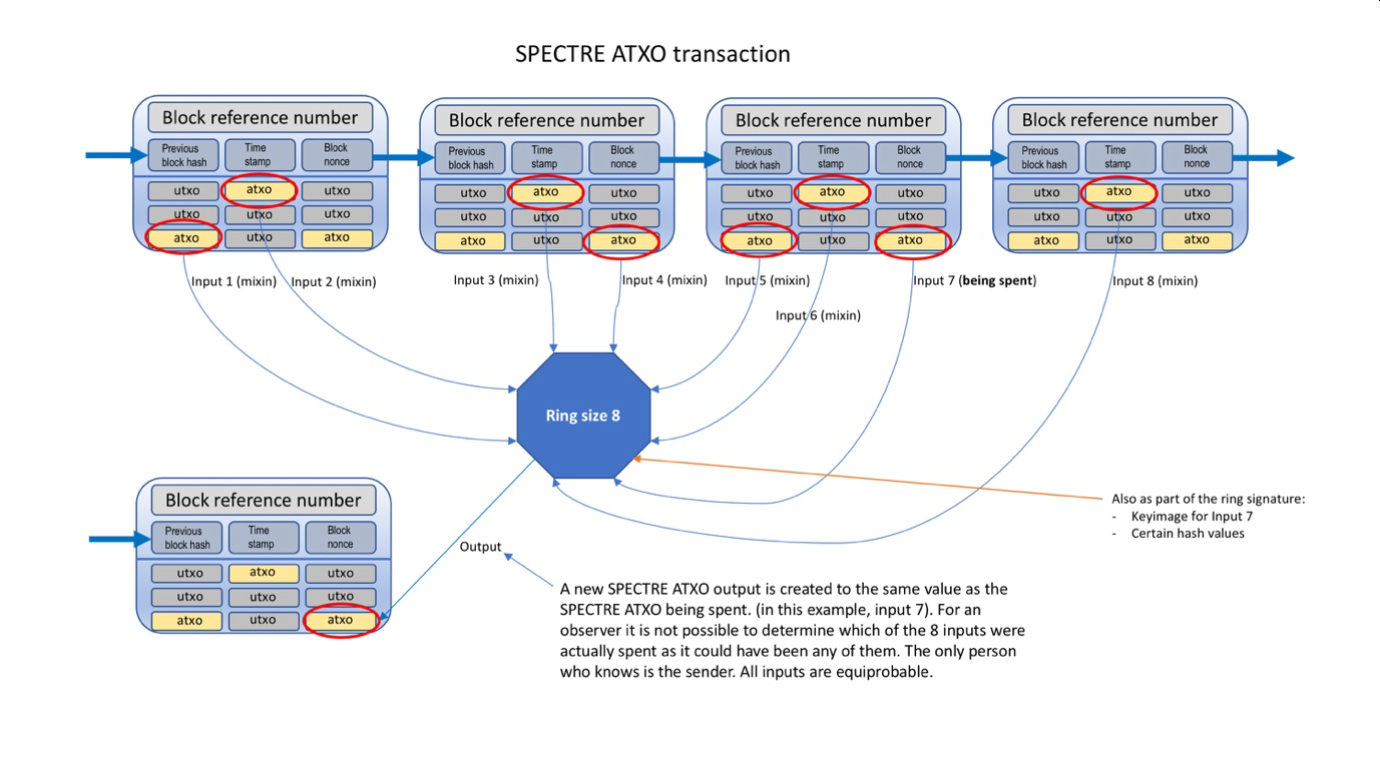
\includegraphics[width=\textwidth]{Anonymous-ATXO-Transaction.png}
	\caption{SPECTRE ATXO transaction}
\end{figure}




\subsection{Minimum Ring Size}

A minimum ring size of 10 is being enforced as part of the consensus since 
Spectrecoin v3.x.
\\
\\
\noindent
Any ATXO used in a ring size 1 transaction will be marked as 
‘\textit{compromised}’ and will not be selected as a ‘\textit{mixin}’ 
in any future ring signature transaction.
\\
\\
\noindent
\textbf{We have seen how dual-key stealth address techniques are used to 
create ATXOs on the Spectrecoin blockchain with bundled one-time key pair 
that can only be ‘spent’ by providing a valid ring signature. In this way 
Spectrecoin protects the privacy of both the sender and the receiver.}



\subsection{Ring-Signature formula}
Spectrecoin uses a ring-signature formula developed by Dr. Adam Back. He 
created a formula based on the traceable ring signature described in the 
CryptoNote white-paper\footnote{https://cryptonote.org/whitepaper.pdf} 
using maths based on the paper "\textit{1-out-of-n Signatures from a Variety of Keys}"\footnote{https://www.researchgate.net/publication/221326919\_1-out-of-n\_Signatures\_from\_a\_Variety\_of\_Keys} 
by Abe, Ohkubo and Suzuki. He was able to create a linkable ring signature 
which tends to be \sfrac{1}{2} of the size of the CryptoNote ring signature 
as the signature is 3+n values vs. 2+2n values.
\newpage
\noindent
Dr. A. Back showed how to add traceability in a way that made it compatible with CryptoNote\footnote{https://bitcointalk.org/index.php?topic=972541.msg10619684}. 
The original description contains 4 parts (\textbf{KEYGEN}, \textbf{SIG}, 
\textbf{VERIFY}, \textbf{LINK}) and is summarized here for comparison:


\hfill \break\textbf{Definitions}:
 
\begin{tabular}{ll}
	$q$:   & a prime number; $q = 2^{255} - 19$\\
	$d$:   & an element of $\mathbb{F}_q$;. $-121665/121666$ \\
	$E$:   & an elliptic curve equation; $-x^2 + y^2 = 1 + dx^2y^2$ \\
	$G$:   & a base point; $G=(x, -4/5)$ \\
	$l$:   & a prime order of the base point; $l=2^{252}+27742317777372353535851937790883648493$ \\
	$\mathcal{H}_s$:   & a cryptographic hash function $\{0,1\}^* \rightarrow \mathbb{F}_q$ \\
	$\mathcal{H}_p$:   & a deterministic hash function $E(\mathbb{F}_q) \rightarrow E(\mathbb{F}_q)$ \\	
\end{tabular}

\hfill \break


\hfill \break\textbf{KEYGEN}: 
The signer selects a secret key $x \in [1, l-1]$ and calculates a public 
key $P$, as well as the key-image $I$ with the following equations:

\begin{equation}
\begin{split}
P &= xG\\
I &= x\mathcal{H}_p(P)\\ 
\end{split}
\end{equation}

\textbf{SIG}: 
The signer selects a set $S'$ of $n$ other users public keys $P_i$, and 
adds his own public key to the set. 

\begin{equation}
\begin{split}
S &= S' \cup \{P_s\}\\
 &= \{P_i\}, i \in [0..n] \\
\end{split}
\end{equation}

Note that the public key $P_{i=s}$ is the signer's own public key, while 
the others are random selected public keys that will be used in the ring 
signature. The index $s$ is the signer secret index. The signer then pics 
$n+1$ random private keys $q_i$ and $n$ private keys $w_i$.

\begin{equation}
\begin{split}
q_i &\in [1...l],  i \in [0...n] \\
w_i &\in [1...l],  i \in [0...n], i \not= s \\
\end{split}
\end{equation}

Now he computes:

\[
L_i= 
\begin{dcases}
q_iG,& \text{if } i = s\\
q_iG+w_iP_i,              & \text{otherwise}
\end{dcases}
\]

and similarly

\[
R_i= 
\begin{dcases}
q_i\mathcal{H}_p(P_i),& \text{if } i = s\\
q_i\mathcal{H}_p(P_i)+w_iI,              & \text{otherwise}
\end{dcases}
\]

Now he calculates the challenge $c$:

\begin{equation}
\begin{split}
c &= \mathcal{H}_s(m, L_1, ..., L_n, R_1, ..., R_n)\\
\end{split}
\end{equation}

And finally the response 

\[
c_i= 
\begin{dcases}
w_i,& \text{if } i \not= s\\
c-\sum_{i=0}^n c_i \quad mod\quad l,              & \text{otherwise}
\end{dcases}
\]

and similarly

\[
r_i= 
\begin{dcases}
q_i,& \text{if } i \not= s\\
q_i-c_sx \quad mod\quad l,              & \text{otherwise}
\end{dcases}
\]

The resulting signature $\sigma$ is then
\[
\sigma = (I, c_1, ..., c_n, r_1, ..., r_n)
\]

One can immediately see that the signature $\sigma$ from the CryptoNote 
white-paper has $2(n+1)$ values for $c_i$ and $r_i$.

\hfill \break\textbf{VERIFY}: 
The first step is to apply the inverse transformation.

\begin{equation}
\begin{split}
L_i' &= r_iG+c_iP_i\\
R_i' &= r_i*\mathcal{H}_p(P_i)+c_iI\\ 
\end{split}
\end{equation}

A verifier now checks that the following condition holds:

\begin{equation}
\begin{split}
\sum_{i=0}^n c_i &\stackrel{?}{=}	 \mathcal{H}_s(m, L_0', ..., L_n', R_0', R_n')
\end{split}
\end{equation}

\hfill \break\textbf{LINK}: 
This step is only applied when the previous step succeeds. The verifier 
uses a set $\mathcal{I}$ of previous signatures and rejects the signature 
$\sigma = (I,... )$ if $I \in \mathcal{I}$.

\hfill \break Dr. Adam Back's variation, and the version of the ring-signature 
algorithm used by spectrecoin, is as follows:

\hfill \break\textbf{KEYGEN}: Like above, pick a random private key 
$x \in [1..l-1]$ and calculate:

\begin{equation}
\begin{split}
P &= xG\\
I &= x\mathcal{H}_p(P)\\ 
\end{split}
\end{equation}

\hfill \break\textbf{SIG}: Pick $n$ random public keys $P_i$ from other 
users, generate $n$ random private keys $s_i \in [1...l-1]$ as well as a 
private key $\alpha \in [1..l-1]$ for the signer with index $j, 0<=j<=n$. 
This gives you the following structure:

\begin{equation}
\begin{split}
\textbf{public keys} &: [P_0, ... P_j, ..., P_n] \\
\textbf{private keys} &: [s_0, ... s_j, ..., s_n] \\
\end{split}
\end{equation}

\hfill \break NOTE that $s_j$ is to be calculated (see below) and $P_j$ 
is the public key of the signer. The next step is to calculate the parameters 
$c_i$ recursively yielding the vector $[c_0, ... ,c_j, ..., c_n]$.

\begin{equation}
\begin{split}
  c_{j+1} & = \mathcal{H}_s(P_1, ..., P_n, \alpha G, \alpha \mathcal{H}_p(P_j))\\
  c_{j+2} & = \mathcal{H}_s(P_1,...,P_n,s_{j+1}G+c_{j+1}P_{j+1},s_{j+1}\mathcal{H}_p(P_{j+1})+c_{j+1}I_j)\\
	      & ... \\
  c_{j} & = \mathcal{H}_s(P_1,...,P_n,s_{j-1}G+c_{j-1}P_{j-1},s_{j-1}\mathcal{H}_p(P_{j-1})+c_{j-1}I_j) \\
\end{split}
\end{equation}

\hfill \break The formula shows that we start to calculate at the position 
$j+1$ , where $j$ represents the signer's index. To keep the index $i$ of 
$c_i$ within the allowed range, we have to take the $mod$ of the number of 
signers. Effectively we calculate the sequence 
$c_{j+1}, c_{j+2}, ..., c_n, c_0, c_1, ... c_j$
 
\hfill \break Next is to find the $s_j$ value: Adam argues that since 
$\alpha G = s_jG+c_jP_j$ , then $\alpha = s_j+c_jx_j$ or 
$s_j = \alpha - c_jx_j\quad mod\quad n.$

\hfill \break The signature $\sigma$ based on this approach is than given 
by $\sigma = (m,I_j,c_1,s_1,...,s_n)$

\hfill \break\textbf{VERIFY}: 

We compute the following equation $\forall_{i=1..n}$

\begin{equation}
\begin{split}
 e_i &= s_iG+c_iP_i \\
 E_i &= s_i\mathcal{H}_p(P_i)+c_iI_j \\
 c_{i+1} &=\mathcal{H}_s(P_1,...,P_n,e_i,E_i)
\end{split}
\end{equation}

Then we check if $c_{n+1}=c_1$.

\hfill \break\textbf{LINK}: 
Like above, we reject duplicate $I_j$ values.


\hfill \break As we can see from the new signature $\sigma = 
(m,I_j,c_1,s_1,...,s_n)$, this version of the ring signature 
uses only 1/2 of the size of the Cryptonote ring signature.
\newpage

\subsection{The ‘All\_Spent’ Dilemma}
A ‘\textit{special}‘ situation could occur where all the ATXOs available for a
certain denomination are spent except for your own ATXO to be used in a transaction.
We are referring to this situation as the \textbf{\textit{‘ALL\_SPENT’ dilemma}}
and although this appears to be a very low probability situation in V3 it could
have dire consequences for privacy and compromise a number of ATXOs. Let’s first
explain this dilemma in some detail:
\\
\\
\noindent
A valid ring signature (\textit{assume ring size 10}) needs: \textbf{(1)} An
unspent ATXO of a certain denomination to be used/spent in the transaction,
and \textbf{(2)} Nine (9) ‘\textit{mixins}’ of the same denomination
(\textit{spent or unspent}). These ‘\textit{mixins}’ (ATXOs) of the same
value as the one being spent provides ‘\textit{plausible deniability}’ with
regards to the sender. The sender could own any one of the ten ATXOs used
in the ring-signature and an observer can not determine which one of the
10 ATXOs forming the ring-signature is being spent. This is at the core of
ring-signature privacy and needs to be preserved.
\\
\\
\noindent
ATXOs of each denomination are “\textit{scattered}” along the Spectrecoin
blockchain and exist in various blocks where they were once created and
they can all be used as ‘\textit{mixins}’ in a ring-signature whether they
have ever been spent or not. Each ATXO is a ‘\textit{unique unit of data}’
identified by its associated ‘\textit{public key}’. However, only the
owner of an ATXO can determine if an ATXO value has been spent or not
as this requires the corresponding ‘\textit{private key}’.
\\
\\
\noindent
The ATXO picking algorithm for a ring-signature selects 9 ‘\textit{mixins}’
at random from the available pool of ATXOs. In each block there could be a
number of ATXOs of different denominations (\textit{spent or unspent})
that could be selected as the 9 ‘\textit{mixins}’.
\\
\\
\noindent
Any observer will be able to establish the following: \textbf{(1)} In each
valid ring-signature on the blockchain there will be one and only one ATXO
of a certain denomination being spent. \textbf{(2)} In each valid
ring-signature there will be nine ‘\textit{mixins}’ used of the same
denomination. \textbf{(3)} The observer will be able to count the number
of existing ATXOs for each denomination by scanning the blockchain.
\textbf{(4)} The observer will be able to count the number of ATXOs for
each denomination that has been spent by counting the number of valid
ring-signatures where this denomination has been used.
\\
\\
\noindent
As a result, if the ‘ALL\_SPENT‘ situation occurs, i.e.:
\\
\noindent
$(number\_of\_\_existing\_ATXOs = number\_of\_spent\_ATXOs)$
\\
\\
\noindent
An observer will be able to categorically determine that each of the ATXOs
used as a ‘\textit{mixin}‘ in the ring-signature has previously been spent.
The sender’s privacy has been compromised as the ‘\textit{real}‘ input ATXO
can be identified, and we no longer have the ‘\textit{plausible deniability}’
afforded by the ring-signature. It is important to point out the following
regarding this issue:



\begin{itemize}
	\item This only occurs when ALL the ATXOs of a denomination have been
	spent and a new transaction is created using the depleted denomination.
	\item The privacy of the transaction spending the last unspent ATXO,
	although creating an ‘ALL\_SPENT‘ situation is not compromised.
	\item If the ‘ALL\_SPENT’ occurs, it would only compromise transaction
	created after the ‘ALL\_SPENT’. All the previous transactions would still
	retain their privacy.
\end{itemize}



\subsubsection{'ALL\_SPENT' illustration}

\begin{figure}[ht]
    \centering
    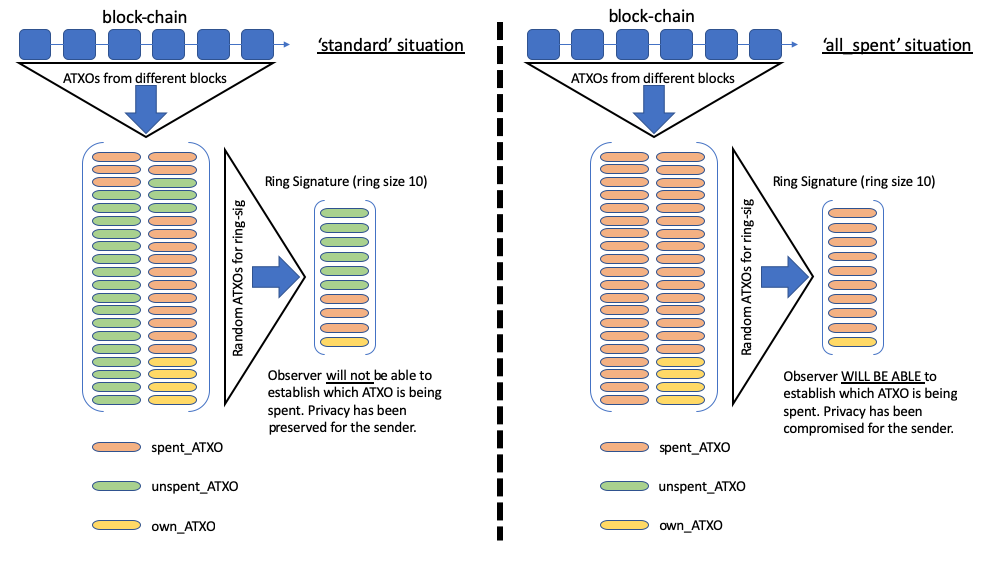
\includegraphics[width=\textwidth]{Images/allspentproblem.png}
    \caption{ALL\_SPENT problem}
    \label{fig:my_label}
\end{figure}

\subsubsection{Solutions}
A range of measures are being implemented to negate the so called
\textit{‘ALL\_SPENT’ dilemma}. We realised that this is only likely
to occur in a situation where there is a very limited supply of
ATXOs of a certain denomination.
\\
\\
\noindent
Therefore, the main approach to solve this problem is to make sure that
there is always a sufficient supply of ATXOs of varying denominations.
We have therefore introduced an advanced ATXO balancer algorithm. This
algorithm will measure the number of ATXO existing for each denomination
and either seek to consolidate ATXO values or split ATXO values as part
of the staking transaction in PoAS. This will ensure that there is
always a sufficient supply of ATXO to act as ‘\textit{mixins}‘.
\\
\\
\noindent
In addition a new algorithm has been implemented to detect an
‘\textit{ALL\_SPENT}‘ situation and if this situation occurs
the network will ‘\textit{remember}‘ the block height (\textit{block number})
and the picking algorithm will no longer pick ‘\textit{mixins}‘
from below that block height. This ensures that users get the full
benefit of the privacy the ring-signature offers.



\subsection{The ‘ATXO\_Set’ Dilemma}

We can say that all the ATXOs created in the same transaction are part
of an ‘\textit{ATXO\_Set}’, i.e. they will forever be linked to each
other as they were created at the same time and it can be assumed that
they all belong to the same user. There will always be multiple outputs
per transaction because of the denomination system, because amounts
have to be split into discrete values.


\noindent
The following dilemma may then occur; the ATXO picking algorithm (as it is
now) could select ATXOs from an ‘\textit{ATXO\_SET}‘ as ‘\textit{mixins}‘
in a ring-signature and this could potentially compromise privacy by making
the signature more susceptible to deductive analysis. In other words, an
observer could be able to determine which of the ‘\textit{mixins}‘ are fake.



\subsubsection{Solutions}
New algorithms have been created to negate these issues and strengthen the
privacy of the network. This way depending on the random pick of the initial
‘\textit{mixins}‘ and the denominations to fill, there will be a random
amount of ‘\textit{mixins}‘ from the same transaction in the final transaction.
\\
\\
\noindent
This will also ensure that each output is only used once as a ‘\textit{mixin}‘
in one of the ring-signatures (VINs). Something which was previously only
assured by chance. Same ‘\textit{mixin}‘ in different VINs can only be fake.



\begin{itemize}
	\item When the first 9 ‘\textit{mixins}‘ for an output are chosen, it is
	completely random, but is ensured that all ‘\textit{mixins}‘ come from
	different transactions.
	\item When ‘\textit{mixins}‘ for the second ring-signature are chosen,
	there is a 33\% chance that the algorithm tries to 	choose outputs from
	the transaction chosen as ‘\textit{mixins}‘ for the first ring-signature.
	If no outputs can 	picked that way, a new random output is chosen and
	the corresponding transaction is added as new source of ‘\textit{mixins}‘.
	\item Repeat.
\end{itemize}


\noindent
We believe that these issues also exist or existed in Monero and other CryptoNote based
systems and may have been described first in a paper entitled
\textit{“A Traceability Analysis of Monero’s Blockchain”}
\footnote{https://eprint.iacr.org/2017/338.pdf} and in particular in
chapter: 5.2 Heuristic II: Leveraging Output Merging in this paper.

\chapter{The Proof-of-Stake (PoSv3) Protocol}
The following section, \underline{in its entirety}, has been taken
directly from, and is based on a blog post by
Qtum\footnote{https://qtum.org/en} developer ‘\textit{Earlz}’
from 27/07/2017 called \textit{“The missing explanation of Proof
of Stake Version 3”}\footnote{http://earlz.net/view/2017/07/27/1904/the-missing-explanation-of-proof-of-stake-version}
and is the best-known source of information on the PoSv3 protocol.
The Spectrecoin PoSv3 implementation adheres completely to this protocol
description for both blocks and transactions and so the explanation from
‘\textit{Earlz}’ can be used for Spectrecoin.



The core concept of Proof-of-Stake (PoS) is very similar to that of
Proof-of-Work (PoW), a lottery. However, the big difference is that,
in PoS, it is not possible to "get more tickets" to the lottery by
simply changing some data in the block and generate a new ticket.
Instead of the "block hash" being the lottery ticket to judge against
a target, PoS invents the notion of a "kernel hash". The ‘kernel hash’
is composed of several pieces of data that are not readily changeable
in the current block. And so, because the miners do not have an easy
way to modify the ‘kernel hash’, they cannot simply iterate through a
large amount of hash values like in PoW. PoS blocks also add many
additional consensus rules in order to realise it's objectives. First,
unlike in PoW, the coinbase transaction (the first transaction in the
block) must be empty and the reward must be 0 tokens. Instead, to reward
stakers, there is a special "staking transaction" which must always be
the 2nd transaction in the block. A ‘staking transaction’ is defined as
any transaction that:


\begin{itemize}
	\item Has at least one valid VIN
	\item It's first VOUT must be an empty script
	\item It's second VOUT must not be empty
\end{itemize}



Furthermore, ‘staking transactions’ must abide by these rules to be valid
in a block:
\begin{itemize}
	\item The second VOUT must be either a pubkey (not pubkeyhash!) script, 
	or an OP\_RETURN script that is unspendable (data-only) but stores data 
	for a public key
	\item The timestamp in the transaction must be equal to the block timestamp
	\item The total output value of a stake transaction must be less than or 
	equal to the total inputs plus the PoS block reward plus the block's 
	total transaction fees. output $<=$ (input + block\_reward + tx\_fees)
	\item The first spent VIN's output must be confirmed by at least 450 
	blocks (in other words, the coins being spent must be at least 450 
	blocks old)
	\item Though more VINs can used and spent in a ‘staking transaction’, 
	the first VIN is the only one used for consensus parameters
\end{itemize}



These rules ensure that the stake transaction is easy to identify and
ensures that it gives enough info to the blockchain to validate the block.
The empty VOUT method is not the only way staking transactions could have
been identified, but this was the original design from Sunny
King\footnote{https://whitepaperdatabase.com/peercoin-ppc-whitepaper/}
and has worked well enough. Now we understand what a ‘staking transaction’
is, and what rules such transaction must abide by.



The next part is to understand the rules for PoSv3 blocks:
\begin{itemize}
	\item Must have exactly 1 staking transaction.
	\item The staking transaction must be the second transaction in the block.
	\item The coinbase transaction must have 0 output value and a single empty VOUT
	\item The block timestamp must have its bottom 4 bits set to 0 (referred 
	to as a "mask" in the source code). This effectively means the blocktime 
	can only be represented in 16 second intervals, decreasing its granularity
	\item The version of the block must be 7
	\item A block's "kernel hash" must meet the weighted difficulty for PoS
	\item The block hash must be signed by the public key in the staking 
	transaction's second VOUT. The signature data is placed in the block 
	(but is not included in the formal block hash)
	\item The signature stored in the block must be "LowS", which means 
	consisting only of a single piece of data and must be as compressed 
	as possible (no extra leading 0s in the data, or other opcodes)
	\item Most other rules for standard PoW blocks apply (valid merkle 
	hash, valid transactions, timestamp is within time drift allowance, etc)
\end{itemize}



There are a lot of details here that we'll cover in a bit. The most important
part that really makes PoS effective lies in the "kernel hash". The kernel
hash is used similar to PoW (if hash meets difficulty, then block is valid).



However, the kernel hash is not directly modifiable in the context of the
current block. We will first cover exactly what goes into these structures
and mechanisms, and later explain why this design is exactly this way, and
what unexpected consequences can come from minor changes to it



\section{The Proof of Stake Kernel Hash}

\underline{The kernel hash specifically consists of the following exact pieces of data (in order):}

\begin{itemize}
	\item Previous block's "stake modifier" (more detail on this later)
	\item Timestamp from "prevout" transaction (the transaction output that 
	is spent by the first VIN of the staking transaction)
	\item The hash of the prevout transaction
	\item The output number of the prevout (ie, which output of the 
	transaction is spent by the staking transaction)
	\item Current block time, with the bottom 4 bits set to 0 to reduce 
	granularity. This is the only thing that changes during staking process
\end{itemize}



\underline{The stake modifier of a block is a hash of exactly:}
\begin{itemize}
	\item The hash of the prevout transaction in PoS blocks, OR the block 
	hash in PoW blocks.
	\item The previous block's stake modifier (the genesis block's stake 
	modifier is 0)
\end{itemize}



The only way to change the current kernel hash (in order to mine a block), 
is thus to either change your "\textit{prevout}", or to change the current 
block time.



A single wallet typically contains many UTXOs. The balance of the wallet is 
basically the total amount of all the UTXOs that can be spent by the wallet. 
This is of course the same in a PoS wallet. This is important though, because 
any output can be used for staking. One of these outputs are what can become 
the "\textit{prevout}" in a staking transaction to form a valid PoS block.



Finally, there is one more aspect that is changed in the mining process of a 
PoS block. The difficulty is weighted against the number of coins in the 
staking transaction. The PoS difficulty ends up being twice as easy to achieve 
when staking 2 coins, compared to staking just 1 coin.



If this were not the case, then it would encourage creating many tiny UTXOs 
for staking, which would bloat the size of the blockchain and ultimately 
cause the entire network to require more resources to maintain, as well as 
potentially compromise the blockchain's overall security.



So, if we were to show some pseudo-code for finding a valid kernel hash now, 
it would look like:



\vspace{5mm} %5mm vertical space

\lstinputlisting{snippets/kernelHashPseudoCode.txt}

\vspace{5mm} %5mm vertical space



This code isn't so easy to understand as our PoW example, so I'll attempt to 
explain it in plain English:



Do the following over and over for infinity:
Calculate the blockTime to be the current time minus itself modulus 16
(modulus is like dividing by 16, but then only instead of taking the
result, taking the remainder)
Calculate the posDifficulty as the network difficulty, multiplied by the
number of coins held by the UTXO.
Cycle through each UTXO in the wallet. With each UTXO, calculate a SHA256
hash using the previous block's stake modifier, as well as some data from
the the UTXO, and finally the blockTime. Compare this hash to the
posDifficulty. If the hash is less than the posDifficulty, then the kernel
hash is valid and you can create a new block.
After going through all UTXOs, if no hash produced is less than the
posDifficulty, then wait 16 seconds and do it all over again.



Now that we have found a valid kernel hash using one of the UTXOs we can 
spend, we can create a staking transaction. This staking transaction will 
have 1 VIN, which spends the UTXO we found that has a valid kernel hash. 
It will have (\textit{at least}) 2 VOUTs. The first VOUT will be empty, 
identifying to the blockchain that it is a staking transaction. The second 
VOUT will either contain an OP\_RETURN data transaction that contains a single 
public key, or it will contain a pay-to-pubkey script. The latter is usually 
used for simplicity but using a data transaction for this allows for some 
advanced use cases (such as a separate block signing machine) without 
needlessly cluttering the UTXO set.



Finally, any transactions from the mempool are added to the block. The only 
thing left to do now is to create a signature, proving that we have approved 
the otherwise valid PoS block. The signature must use the public key that is 
encoded (either as pay-pubkey script, or as a data OP\_RETURN script) in the 
second VOUT of the staking transaction. The actual data signed in the block 
hash. After the signature is applied, the block can be broadcast to the 
network. Nodes in the network will then validate the block and if it finds 
it valid and there is no better blockchain then it will accept it into its 
own blockchain and broadcast the block to all the nodes it has connection to.



It is highly recommended that you read the blog post by
‘\textit{Earlz}’\footnote{http://earlz.net/view/2017/07/27/1904/the-missing-explanation-of-proof-of-stake-version} 
and also the associated white papers for
PoS\footnote{https://whitepaperdatabase.com/peercoin-ppc-whitepaper/} and
PoSv2\footnote{https://blackcoin.org/blackcoin-pos-protocol-v2-whitepaper.pdf} 
if you want to fully understand how Proof-of-Stake works. PoSv3 as described 
here also forms the basis of Proof-of-Anonymous-Stake that we will explore a 
bit further on.

\chapter{The Proof-of-Anonymous-Stake (PoAS) protocol}
This section introduces a new staking algorithm that was introduced to the 
Spectrecoin mainnet through the release of v3.0.9 and a hard-fork on 
17\textsuperscript{th} May 2019. This is the first known implementation 
of a private staking protocol employing ring-signatures in the staking 
transactions. This protocol was designed and coded by Spectrecoin lead 
developer Philip Mueller (\textit{@Tek}). The protocol is based on the 
PoSv3 protocol that we described in the previous section.



\section{Introduction}
We consider that a privacy focused pure Proof-of-Stake (\textit{PoS}) 
network such as Spectrecoin need to be able to maintain consensus through 
a mechanism that maintains privacy, prevents easy blockchain analysis and 
is censorship resistant. Hence, such a network is not complete without a 
way to stake in private. There should be a way to maintain the privacy of 
all the network participants throughout the staking process. The 
participants should also be able to acquire their stake reward whilst 
maintaining their privacy.



\section{The Problem}

In a standard staking transaction (\textit{PoSv3}) a value known as the '\textit{kernel hash}' is calculated from several inputs including values taken from the last valid block, called a '\textit{StakeModifier}' and the value of the user's UTXO. A valid '\textit{kernel hash}' needs to be below a certain threshold that is determined by a separate calculation. The user (the wallet) who is able to generate a valid 'kernel hash' will be granted the right to add the next block to the block-chain. The newly added block includes the generated stake reward (XSPEC) and any transactions currently in the memory pool + any fees. The UTXO used to calculate the valid 'kernel hash' will be spent and the generated stake reward + the value of the spent UTXO will be included in a newly generated UTXO associated with the same public address. In this way every stake that has been generated as a result of UTXOs associated with a certain public address will forever be linked to that address and it's plain for all to see. Below is an example of a standard staking transaction: Example of a staking transaction from the Spectrecoin block explorer\footnote{https://chainz.cryptoid.info/xspec/block.dws?1190944.htm} As with any typical PoS cryptocurrency the staking transactions suffer from all the privacy issues of a standard UTXO transaction, and these transactions are potentially traceable and linkable on the blockchain. It would therefore require some effort from the users to try to maintain anonymity in a standard PoS system and that will in turn weaken the overall resilience of the network against analysis. The network should not have to depend on the participants to maintain anonymity. All the staking transactions completed by the same user can potentially be linked and users’ balances can be estimated, hence the ‘rich list’ feature of many block explorers. As explained previously, most block-chain forensic analysis focuses on address re-use and change addresses and this is exactly what you get with a standard PoS network.



\section{The Solution}
We have therefore developed what we call ‘Proof-of-Anonymous-Stake’ (PoAS) to solve this problem. This is a brand new and novel staking protocol utilising only SPECTRE and ring-signatures in the staking transactions and the rewards are also paid in SPECTRE. This offers a through-and-through confidential way to maintain consensus and provide strong privacy for participants whilst securing the network. It is also appropriate to emphasise that this confidential and private consensus mechanism is totally decentralised and do not depend on any central servers or authority and is 100% peer-to-peer and there is no trusted setup. This provides very strong network resilience with no single point of failure.



\section{Benefits of Anonymous Staking}
The benefits are straight forward and easy to appreciate; if you transfer your holdings to SPECTRE, our anonymous coin, nobody will be able to know your balance, nobody will know how much you stake and if you keep transactions SPECTRE <> SPECTRE you preserve your privacy at all times. It is useful however to remember that once SPECTRE is converted to XSPEC all your XSPEC <> XSPEC transactions are again potentially traceable. Note that the potential traceability only becomes an issue after the conversion from SPECTRE >> XSPEC and does not affect the previous SPECTRE transaction. With the addition of anonymous staking to Spectrecoin and the updated UI it is now easy to distinguish between the different transactions and you will clearly see if you are staking XSPEC, SPECTRE or both. The previously described ‘Development Contribution Blocks’ (marked as ‘contributed’) will still occur every 1 in 6 blocks regardless of whether the block has been staked via the standard staking transaction or the anonymous ATXO staking transaction.

\section{TOR (The Onion Router)}
TOR aka. ‘\textit{The Onion Router}’ is described on the project
website\footnote{https://www.torproject.org/ } like this; “\textit{Tor is
free software and an open network that helps you defend against traffic
analysis, a form of network surveillance that threatens personal freedom
and privacy, confidential business activities and relationships, and
state security.}”



TOR, in essence, hides your real IP address and instead provides you with
a so called \textit{.onion} address that should be extremely difficult to
de-anonymise for any attacker. A normal IP might look like this: 123.45.67.8
and an \textit{.onion} address might look like this:
\textit{fpzcf23ifxpiucjm.onion}. When you broadcast your normal IP address
it will be possible for an adversary to identify you through your internet
service provider that will hold all the data on all connections. If you
broadcast a .onion address only this is not possible and any traffic can
only be traced back to another hidden node on the TOR network. Spectrecoin
has TOR ‘\textit{built-in}’ and running as a process and when you start the
software you will connect to the TOR network with an \textit{.onion} address
and you will not broadcast your real IP address through the Spectrecoin
software for as long as you use the software. The Spectrecoin network will
reject all non-TOR connections.



We are aware of ongoing discussions about TOR vs. I2P\footnote{https://geti2p.net/en/}
vs. Monero’s Kovri project that is currently under development. You can
read up on this, but it is clear that both may have both advantages and
disadvantages. TOR is in wider use and will have more development effort
behind. We are also aware of technology such as Dandelion and we will keep
an eye on developments in this area of network security and we are
considering this.



If you want yet another layer of network security, you can also use a VPN
service with TOR so explore this if you feel that you need this level of
security.


\subsection{OBFS4}
OBFS4 is what is known as a TOR ‘\textit{pluggable Transport}’ and is a
means to hide the fact that you are connecting using TOR. A range of
countries including China and Iran for example are using technology to
block TOR traffic and we have implemented this to try and circumvent any
such censorship. It’s also useful to bear in mind that some countries might
view a TOR user with suspicion although it’s not blocked. When you go to
the download page for Spectrecoin look for the OBFS4 versions of the
software.



\begin{figure}[h]
	\caption{Spectrecoin wallet version with includet OBFS4}
	\centering
	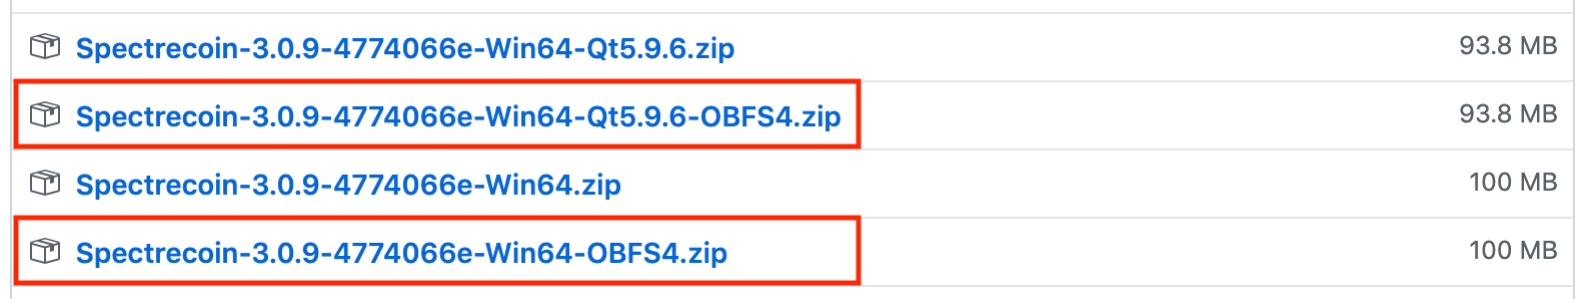
\includegraphics[width=\textwidth]{OBFS4-Walletversions.png}
\end{figure}




It’s difficult to say with 100\% certainty which countries block TOR but
you can find more information on this\footnote{https://metrics.torproject.org/userstats-bridge-table.html}
topic on the TOR project website, that will show you the top 10 countries
where TOR bridges are used. This\footnote{https://grobox.de/tor/} website
may also be of interest and for further information on TOR bridges and
transports you can find a lot of information
here\footnote{https://2019.www.torproject.org/docs/bridges} on the TOR
website and elsewhere. We will be considering various options in this
area in future development.

\section{The Spectrecoin Foundation}
The Spectrecoin Foundation CIC is a UK registered ‘\textit{Community Interest Company}‘.
This means that we are strictly a \textbf{not-for-profit} endeavour focused
on developing and promoting our software, \textbf{Spectrecoin}. The remit
for the foundation also covers an effort to encourage wider adoption and
use of Spectrecoin.
\\
\\
\noindent
We are subject to UK rules, regulation and company law and the foundation
is also responsible for managing the ‘\textbf{\textit{Spectrecoin Development Fund}}‘
to further the aims of the foundation. We are therefore accountable to
the UK authorities with regards to our not-for-profit status and we will
file financial reports just like any other UK company that will be publicly
available. In this way users of Spectrecoin can be confident that any funds
coming into the foundation are used only for product development and
promotion. As the UK has strict laws and regulation around how companies
operate, we feel that we achieve maximum transparency as opposed to a company
registered in some offshore territory or other tax haven with relaxed but
opaque corporate regulation and taxation.



\subsection{Benefits for Users and Investors}
\begin{itemize}
	\item The ‘\textbf{\textit{Spectrecoin Development Fund}}‘ is managed
	within a regulated corporate structure specifically set up to be a
	not-for-profit organisation where the stated objective is to benefit
	the community. This cannot be changed unless the corporation as such
	is dissolved.
	\item The current members of the foundation are dedicated to the long-term
	development of Spectrecoin. The members have a personal stake in the
	project and a responsibility under UK law to manage the funds and further
	the stated aim of the foundation.
	\item There are currently 4 members (\textit{see below}), but members can
	join and members can leave. The foundation in effect ‘\textit{owns}‘ the
	Spectrecoin official GitHub repo and the GitHub organisation and is
	therefore recognised as the only entity that will issue official
	Spectrecoin software. The foundation will also own all the right to the
	web domains and any other Spectrecoin intellectual property. That means
	that even if the original members would leave the foundation, other
	members could join and have 100\% control over Spectrecoin resources in
	the future. The current members would relinquish any control over any
	Spectrecoin asset upon leaving the foundation.
	\item Should the development fund allow, the foundation members could be
	paid up industry standard salaries that would be subject to scrutiny
	under UK law. In this way, there are strict limits to the level of
	renumeration members could receive.
	\item The entirety of the funds will be used for development of the
	software, that could include hiring people or using contractors. Should
	the development fund be of substantial value beyond development costs
	and salaries, any surplus would be used for research grants or funding
	of research into privacy technology or to further the adoption of
	Spectrecoin.
	\item The fact that the foundation and a corporate structure exists
	does not in any way detract from the objective of developing privacy
	focused blockchain technology and does not in any way impose any
	restrictions on our research and development by the UK government.
	(\textit{also see disclaimer}).
\end{itemize}



\subsection{Funding}
The Spectrecoin blockchain forked on 21/08/2018 @ 2200 hours (GMT) to
introduce ‘\textit{Development Contribution Blocks}’ (DCB) to secure a
minimum amount of funding for the project. One in six staking block rewards
will be designated DCBs and will be sent to the Spectrecoin Foundation
wallet for further distribution. One in 6 block rewards means that the
stake reward from block 1, 6, 12, 18 and so forth are designated DCB
regardless of who owns wallet that “\textit{won}” and signed the
contribution block. This means that larger wallets will have a higher
probability of donating. It also means that it is possible to
“\textit{win}” two or more stake rewards 6 blocks apart and the owner
of the wallet will contribute 2 stake rewards in a row. We believe that
this will average out and that on the whole larger wallets will contribute
more. This system can be considered transitional system and we are working
on an improved version of this and we are also exploring ideas around
future funding.
\\
\\
\noindent
This fund will ensure a future for Spectrecoin, will enable us to pay for
certain services, hire contractors and to pay Spectrecoin core team members
in XSPEC/SPECTRE to enable them to work on the project. We believe this
will give us the opportunity to produce better software and will create
value for investors.



\subsection{Members}
The Spectrecoin Foundation currently have 4 directors who are also members,
this is currently the same persons who comprises the Spectrecoin Core team
and they currently responsible for managing and developing Spectrecoin.
They are:



\begin{description}
	\item[Eirik Korsell]  (founder) - https://www.linkedin.com/in/eirik-korsell-37b053173/
	\item[Philip Mueller] (lead developer) - https://www.linkedin.com/in/philip-mueller-82039585/
	\item[Yves Schumann] (developer) - https://www.linkedin.com/in/yves-schumann-02101014b/
	\item[Neil Borum] (community manager) - https://www.linkedin.com/in/neil-borum-bba0b911/
\end{description}





\backmatter
% bibliography, glossary and index would go here.

\end{document}